
\chapter{Crimson vs. Asynchronous Messenger}

\graphicspath{ {../figures} }

\begin{figure}[!ht]
  \centering
  \begin{minipage}{.5\textwidth}
  \centering
    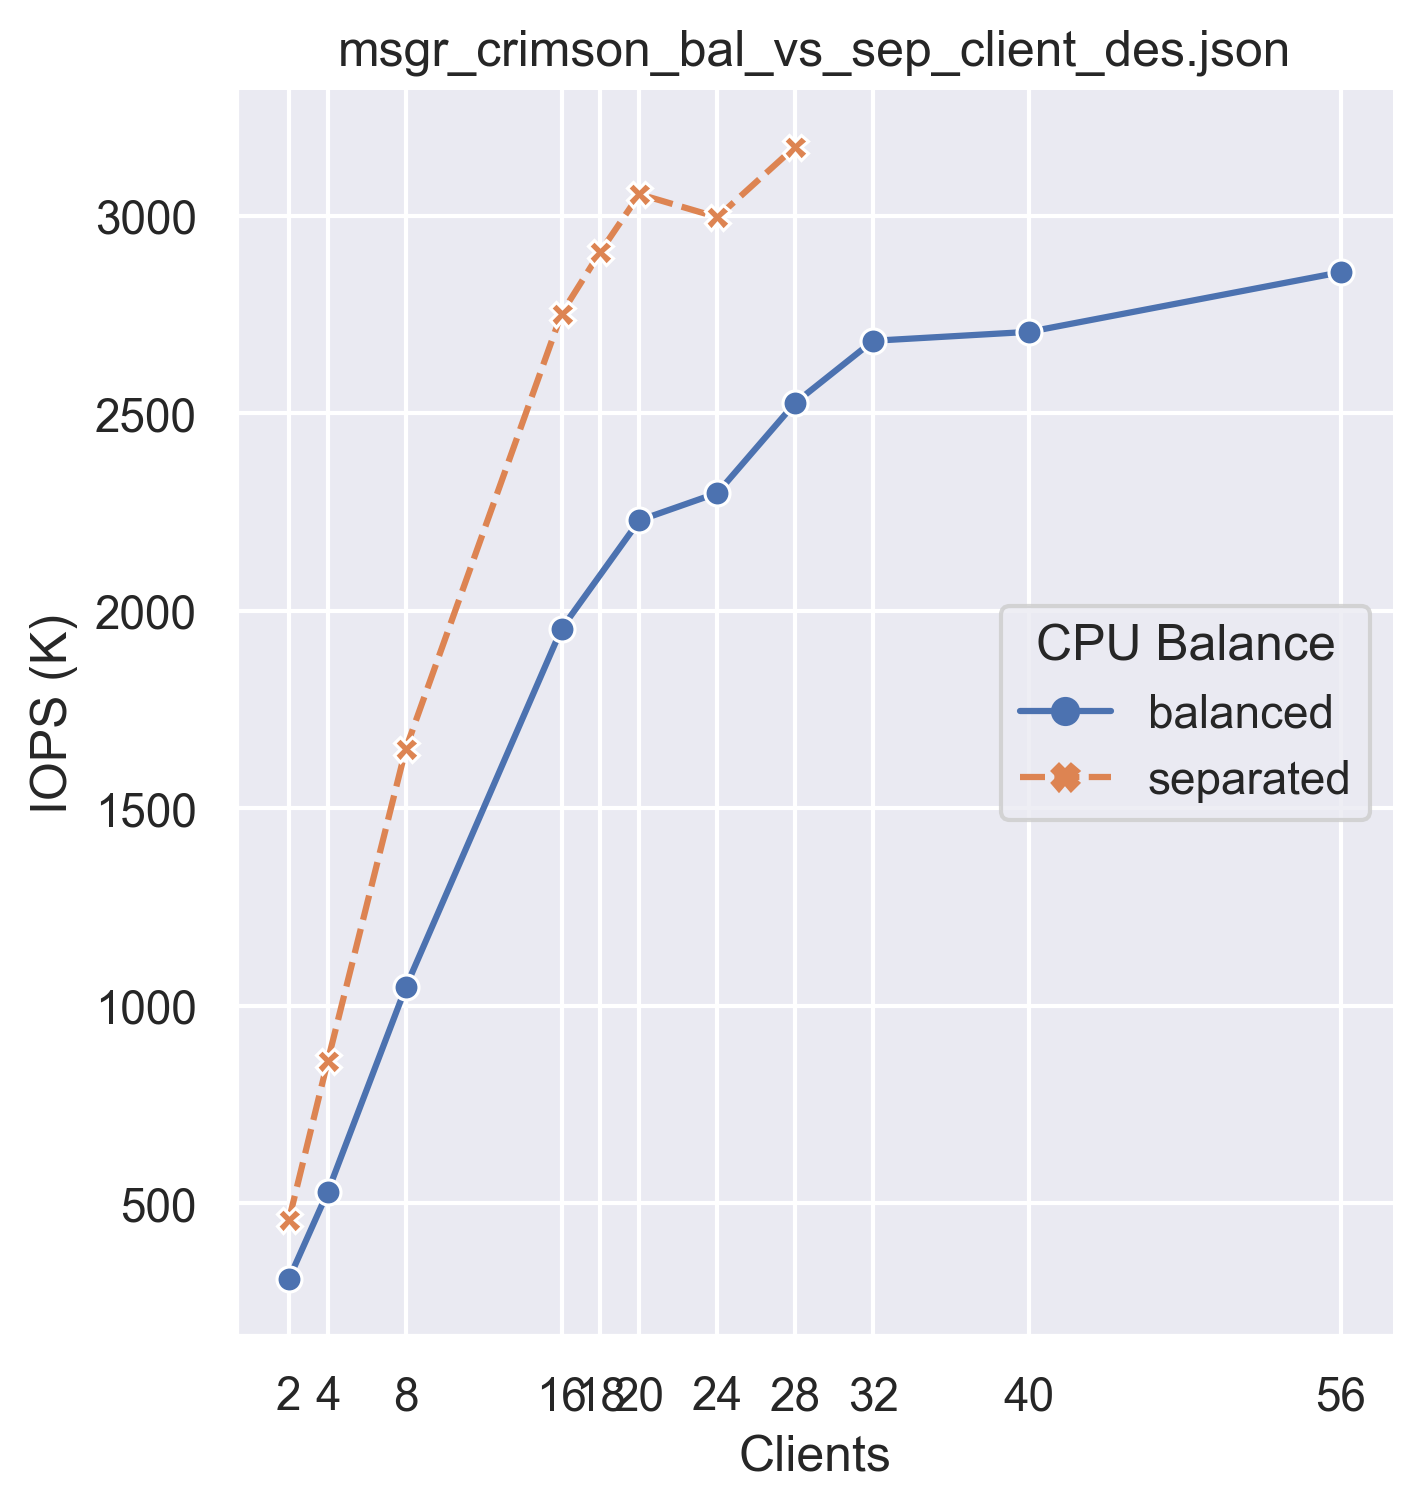
\includegraphics[width=\textwidth]{msgr_crimson_bal_vs_sep_client_des_iops.png}
  \end{minipage}%
  \begin{minipage}{.5\textwidth}
  \centering
    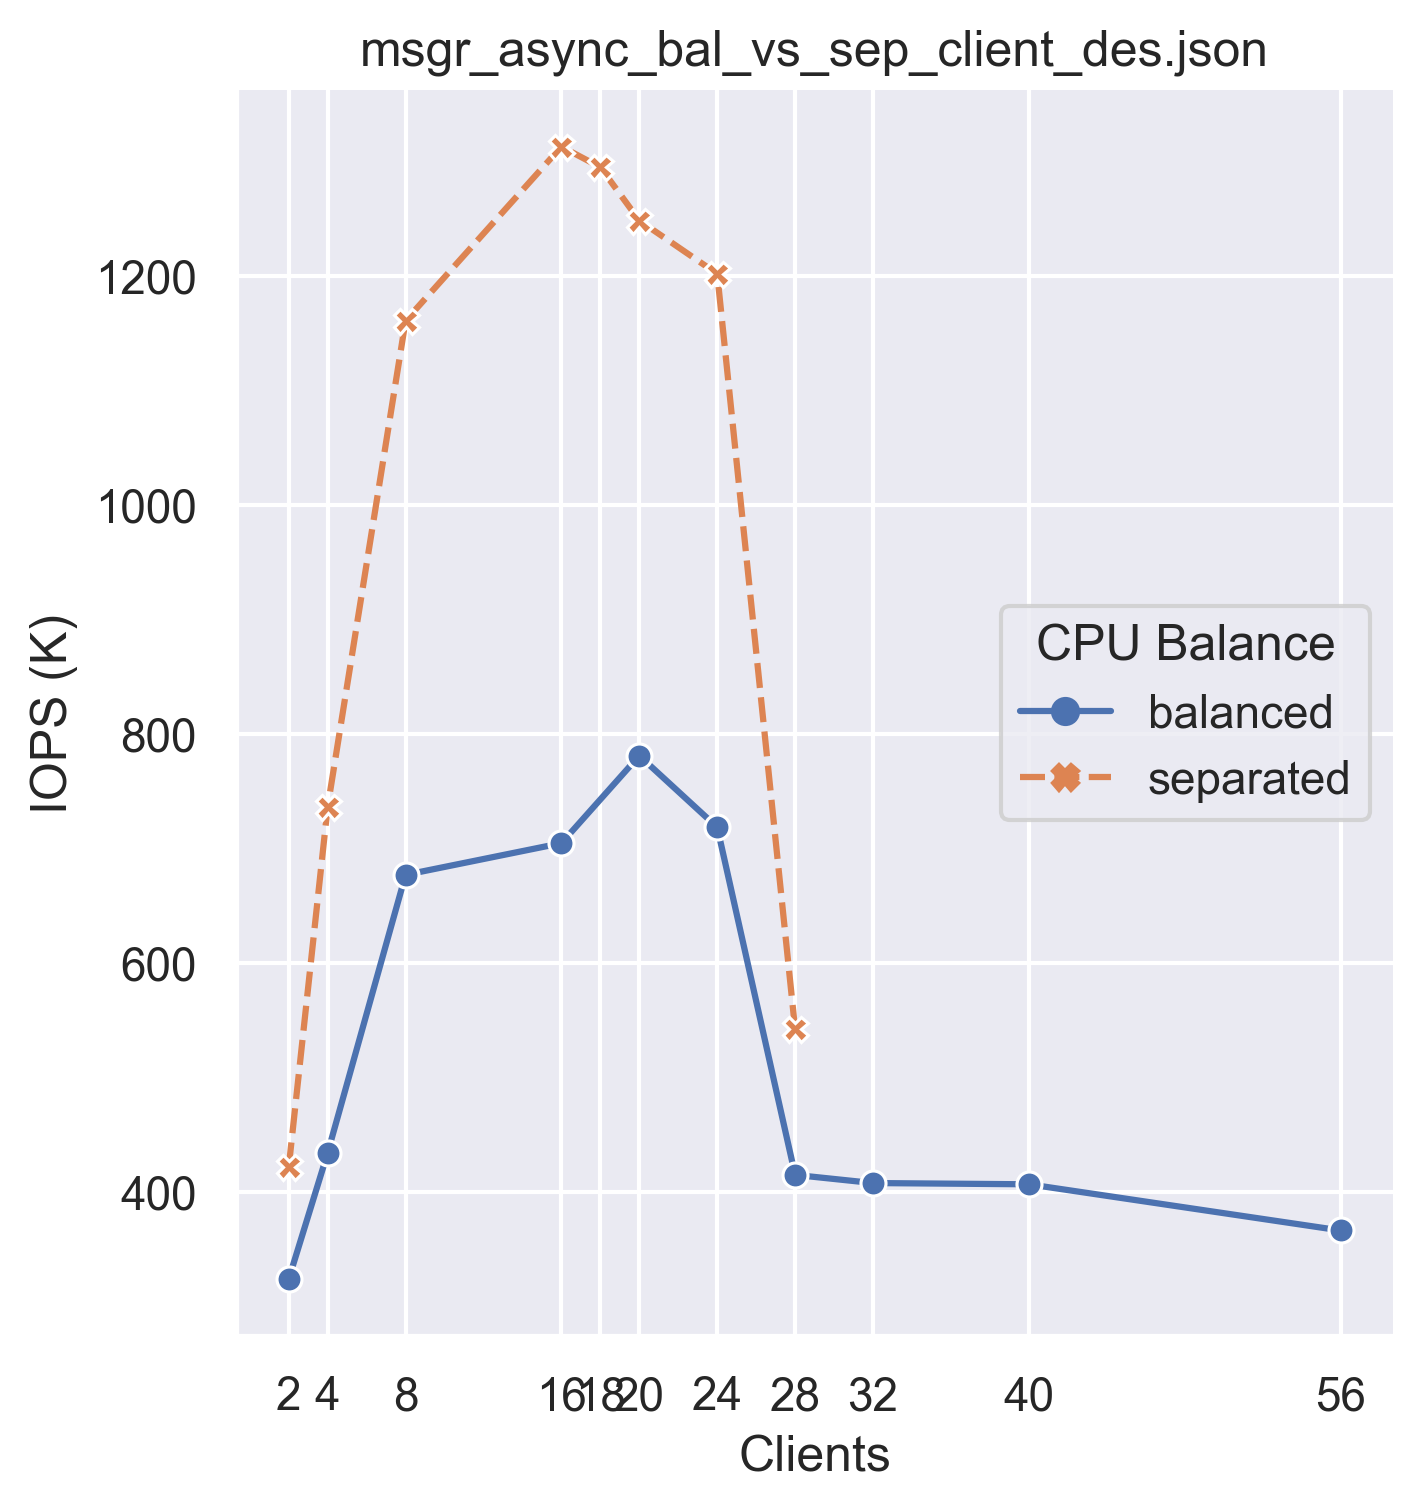
\includegraphics[width=\textwidth]{msgr_async_bal_vs_sep_client_des_iops.png}
  \end{minipage}%
  \caption{Comparison Crimson vs. Async Messenger, across number of clients
  (that matches the number of CPU cores on each server/client process). The CPU
  allocation strategy is described in the text. Note the maximum in linear
  progression for Crimson is reached at 20 clients/cores, whereas for
  Asynchronous the maximum is reached at 16, before dropping. The left-hand
  side shows the results for the Crimson Messenger, while the right-hand side
  shows the results for the Asynchronous Messenger.}
  \label{figure:crimson_vs_async}
\end{figure}

Table \ref{table:crimson-msgr} shows the summary results from the Crimson Messenger clients.
\begin{table}[!h]
\centering
{\small
\begin{tabular}{lrlrlllllr}
\toprule
 & IOPS & balance & clients & connect time & latency & messages received & messaging time & out throughput & smp \\
\midrule
9 & 307.378257 & balanced & 2 & 0.000601 & 6.315879 & 18479209 & 60.118791 & 1200.696318 & 2 \\
10 & 456.714309 & separated & 2 & 0.000537 & 3.767112 & 27495083 & 60.201930 & 1784.040270 & 2 \\
13 & 528.595002 & balanced & 4 & 0.001026 & 7.466761 & 31794168 & 60.148446 & 2064.824228 & 4 \\
14 & 860.158540 & separated & 4 & 0.000651 & 3.763005 & 51835855 & 60.263141 & 3359.994298 & 4 \\
16 & 1046.102510 & balanced & 8 & 0.001477 & 7.468468 & 62980255 & 60.204664 & 4086.337928 & 8 \\
17 & 1649.778424 & separated & 8 & 0.000978 & 3.870238 & 99482787 & 60.300697 & 6444.446968 & 8 \\
0 & 1954.570844 & balanced & 16 & 0.002781 & 7.922822 & 117662783 & 60.198788 & 7635.042360 & 16 \\
1 & 2752.619429 & separated & 16 & 0.001820 & 5.156500 & 165785459 & 60.228254 & 10752.419646 & 16 \\
2 & 2909.627862 & separated & 18 & 0.002174 & 5.787955 & 175092652 & 60.176994 & 11365.733834 & 18 \\
3 & 2229.153323 & balanced & 20 & 0.003867 & 8.765333 & 134374648 & 60.280567 & 8707.630169 & 20 \\
4 & 3054.879799 & separated & 20 & 0.002809 & 6.207968 & 183833595 & 60.177034 & 11933.124215 & 20 \\
5 & 2298.286376 & balanced & 24 & 0.004434 & 10.319926 & 138310138 & 60.179686 & 8977.681158 & 24 \\
6 & 2996.773003 & separated & 24 & 0.003162 & 7.728365 & 180348405 & 60.180873 & 11706.144545 & 24 \\
7 & 2526.839747 & balanced & 28 & 0.004654 & 10.910158 & 152236774 & 60.247898 & 9870.467762 & 28 \\
8 & 3175.492177 & separated & 28 & 0.003748 & 8.430074 & 191154296 & 60.196743 & 12404.266318 & 28 \\
11 & 2683.741510 & balanced & 32 & 0.005687 & 11.925058 & 161478779 & 60.169266 & 10483.365273 & 32 \\
12 & 2706.409334 & balanced & 40 & 0.007641 & 15.021456 & 162852694 & 60.172969 & 10571.911462 & 40 \\
15 & 2857.408738 & balanced & 56 & 0.013819 & 19.216298 & 172858700 & 60.494839 & 11161.752882 & 56 \\
\bottomrule
\end{tabular}


}
\label{table:crimson-msgr}
\caption{Summary of the results for the Crimson Messenger. The table shows the
  number of clients, the CPU core allocation strategy (Balanced or Separated),
  the IOPS and latency in milliseconds.}
\end{table}

In Figure \ref{figure:crimson_vs_async-rc}, we show the comparison using latency response curves.

\begin{figure}[!ht]
  \centering
  \begin{minipage}{.5\textwidth}
  \centering
    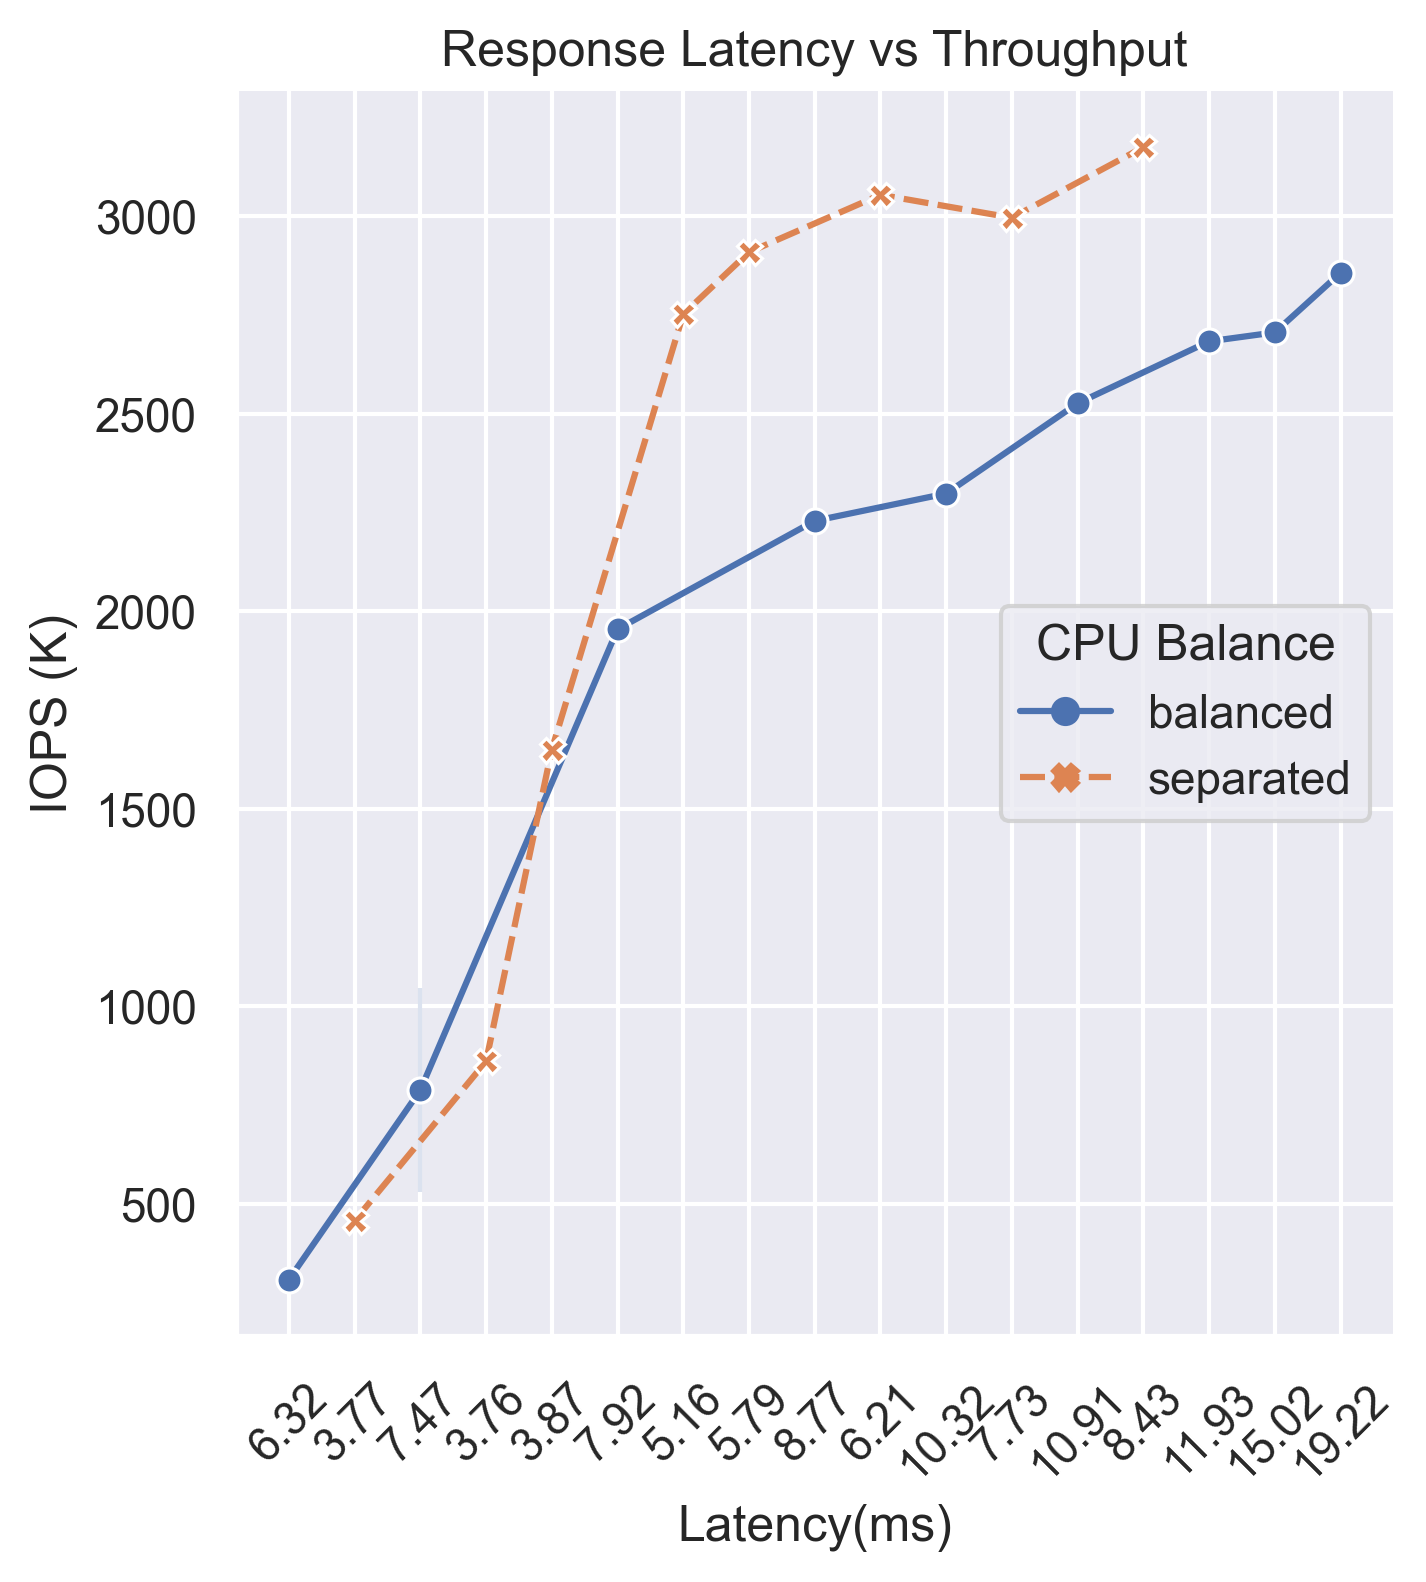
\includegraphics[width=\textwidth]{msgr_crimson_bal_vs_sep_client_des_rc.png}
  \end{minipage}%
  \begin{minipage}{.5\textwidth}
  \centering
    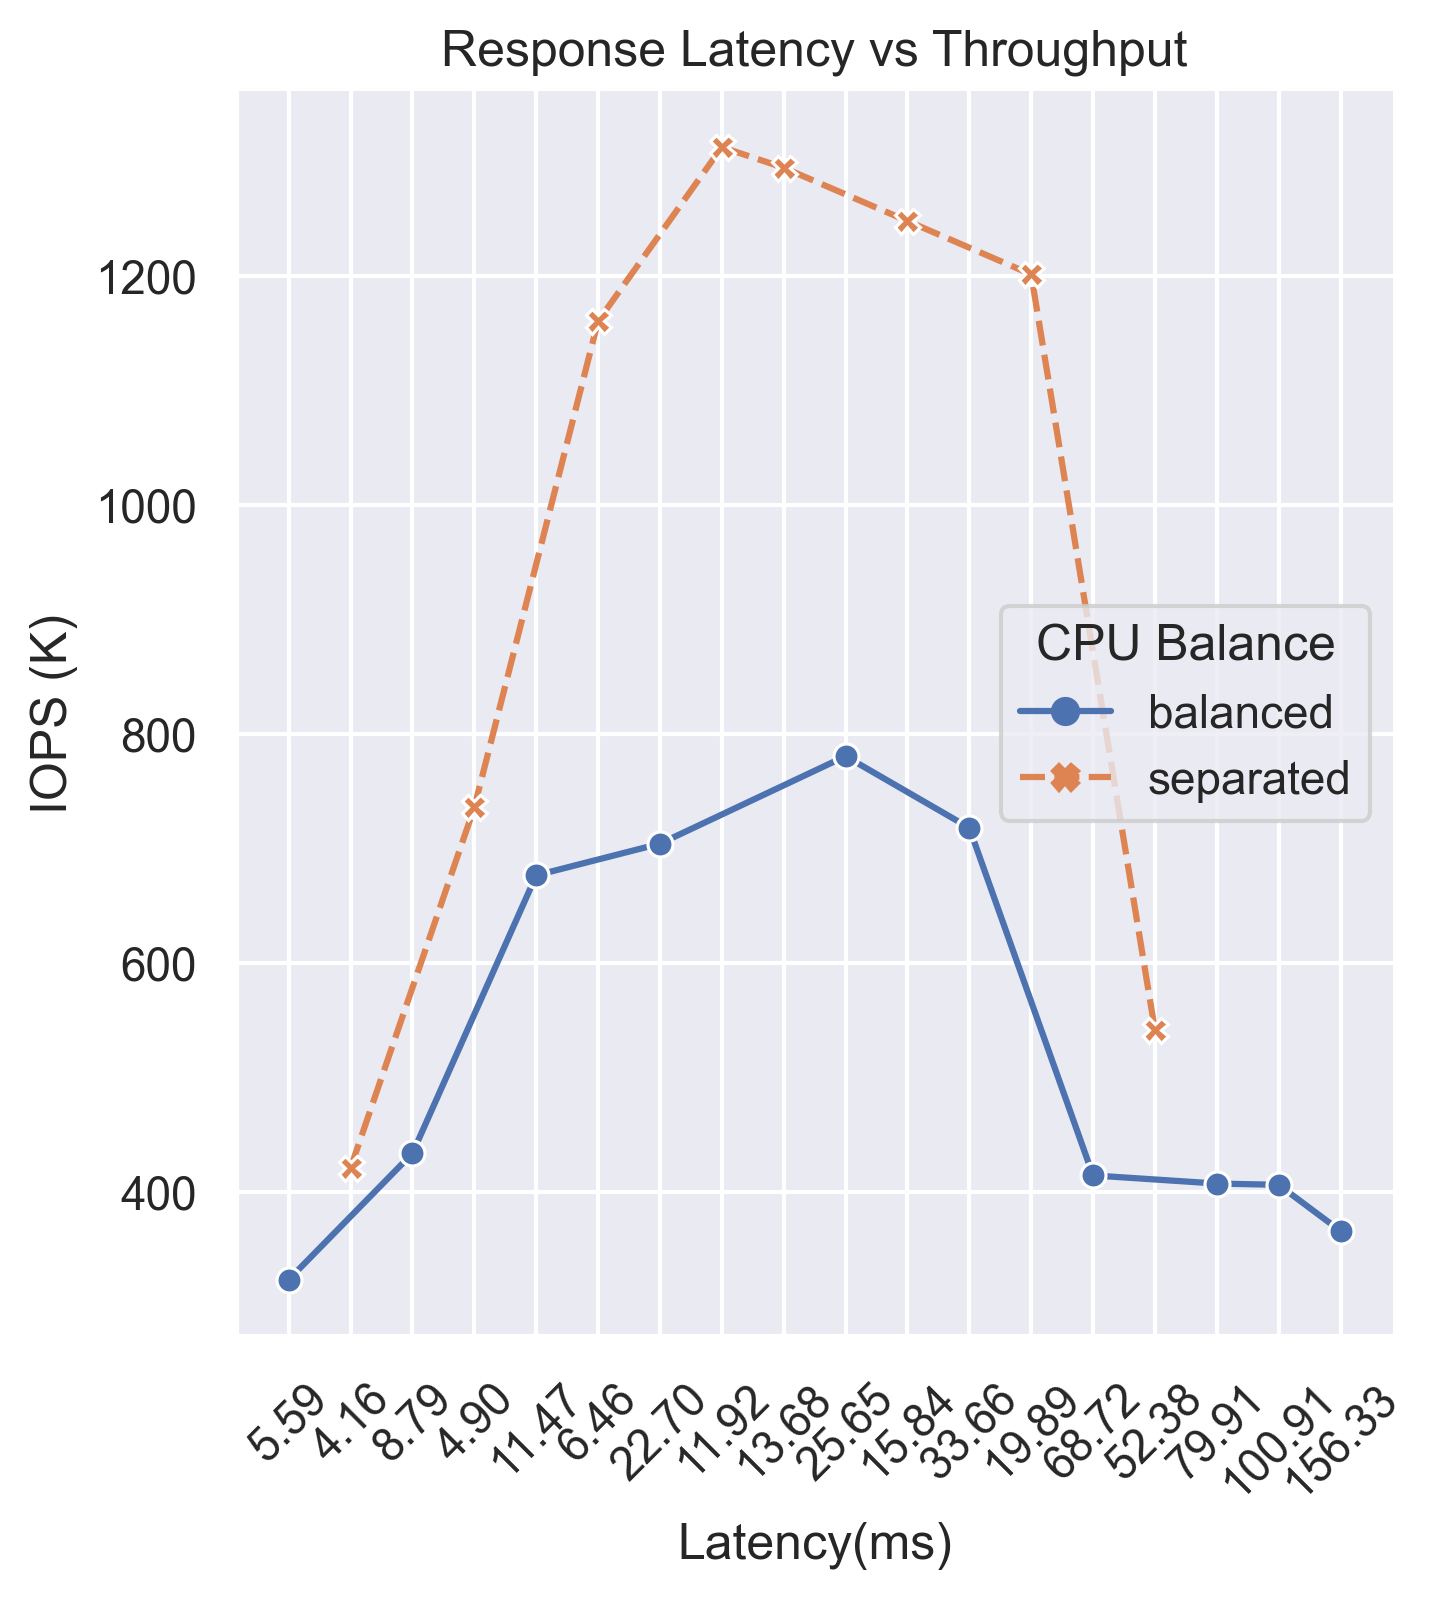
\includegraphics[width=\textwidth]{msgr_async_bal_vs_sep_client_des_rc.png}
  \end{minipage}%
  \caption{Response latency curves for the comparison Crimson vs. Async Messenger.}
  \label{figure:crimson_vs_async-rc}
\end{figure}


% In this Chapter, we show the performance results via latency response curves
% for the comparison between the Crimson and Asynchronous Messenger.
\section{Background}

We first describe the standalones used for the test comparison, then we
summarise the CPU core allocation Balanced vs. Separated.
\begin{description}
\item [Crimson Messenger] we used the
  standalone \texttt{perf-crimson-msgr} for server and client, as shown in Listing \ref{lst:crimson}.

\begin{lstlisting}[language=sh, caption=Invocation of the Crimson Messenger, label=lst:crimson]
# Crimson messenger: seastar cpuset overrides --smp=${SMP}
test_row["server"]="/ceph/build/bin/perf-crimson-msgr --poll-mode --mode=2 --server-fixed-cpu=0\
  --cpuset=${SERVER_CPU_CORES}"
test_row['client']="/ceph/build/bin/perf-crimson-msgr --poll-mode --mode=1 --depth=512\
  --clients=${num_clients} --conns-per-client=2  --cpuset=${CLIENT_CPU_CORES} \
  --msgtime=60 --client-skip-core-0=0"
\end{lstlisting}

\item [Asynchronous Messenger] we used the standalone \texttt{perf-async-msgr}
for server and \texttt{perf-crimson-msgr} for client, as shown in Listing \ref{lst:async}. 

\begin{lstlisting}[language=sh, caption=Invocation of the Asynchronous Messenger, label=lst:async]
# Async messenger: only the server is async, client is crimson
test_row["server"]="taskset -ac ${SERVER_CPU_CORES} /ceph/build/bin/perf-async-msgr --threads=${SMP}"
test_row['client']="/ceph/build/bin/perf-crimson-msgr --poll-mode --mode=1 --depth=512\
  --clients=${num_clients} --conns-per-client=2 --cpuset=${CLIENT_CPU_CORES} --msgtime=60\
  --client-skip-core-0=0"
\end{lstlisting}

\end{description}

The test is executed ranging over the number of clients, which matches the
associated number of CPU cores. We have two major cases for the CPU core
affinity of the clients and the server, respectively:
\begin{itemize}
\item \textbf{Balanced}: the server and client are pinned to the CPU cores
using both a physical and its HT-sibling, on both NUMA sockets.
\item \textbf{Separated}: the server  and client are pinned to physical cores only, 
each on a separate NUMA socket.
\end{itemize}
This is best illustrated in the JSON configuration file shown in Listing
\ref{lst:table-cpu}, where the number of CPU cores (and hence clients) are
listed as keys for each dictionary, their value is the string represented the
range of CPU code ids to be used as argument to the \texttt{cpuset} option, and
\texttt{taskset}, as appropriate.

\begin{lstlisting}[language={[3]Python}, caption=Range of clients and their CPU set, label=lst:table-cpu]
{
"balanced": {
  "server": {
    "2": "0,56",
    "4": "0,56,28,84",
    "8": "0-1,56-57,28-29,84-85",
    "16": "0-3,56-59,28-31,84-87",
    "28": "0-6,56-62,28-34,84-90",
    "32": "0-7,56-63,28-35,84-91",
    "40": "0-9,56-65,28-37,84-93",
    "56": "0-13,56-69,28-41,84-97"
  },
  "client": {
    "2": "1,57",
    "4": "1,57,29,85",
    "8": "2-3,58-59,30-31,86-87",
    "16": "4-7,60-63,32-35,88-91",
    "28": "7-13,63-69,35-41,91-97",
    "32": "8-15,64-71,36-43,92-99",
    "40": "10-19,66-75,38-47,94-103",
    "56": "14-27,70-83,42-55,98-111"
  }
},
"separated": {
  "server": {
    "2": "0-1",
    "4": "0-3",
    "8": "0-7",
    "16": "0-15",
    "28": "0-27"
  },
  "client": {
    "2": "28-29",
    "4": "28-31",
    "8": "28-35",
    "16": "28-43",
    "28": "28-55"
  }
}
}
\end{lstlisting}

We show the extreme configurations for the Balanced CPU core allocation for
Crimson in Figures~\ref{figure:crimson_bal_2} and \ref{figure:crimson_bal_56}.

\begin{figure}[!ht]
  \centering
  \begin{minipage}{.5\textwidth}
  \centering
    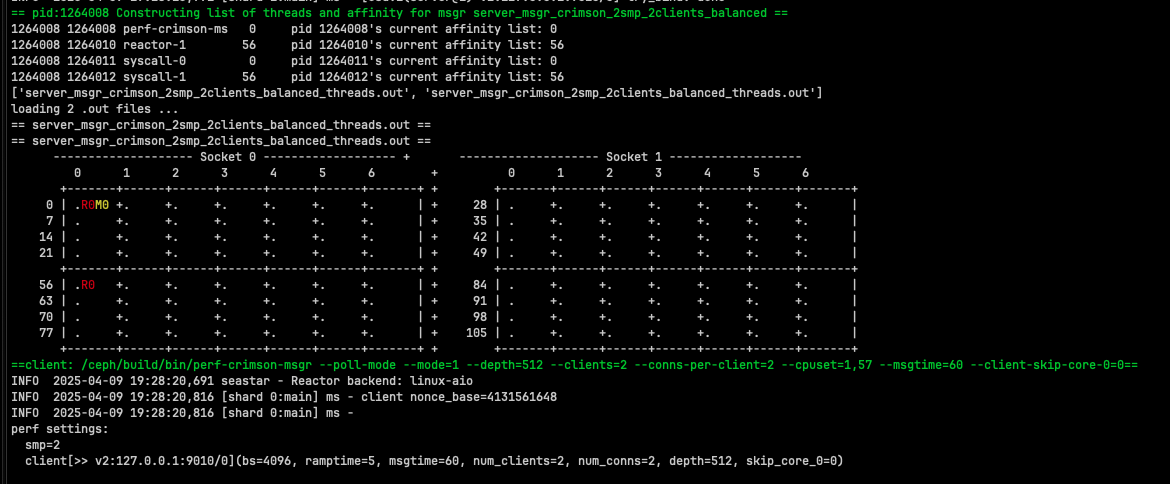
\includegraphics[width=\textwidth]{server_msgr_crimson_2smp_2clients_balanced.png}
  \end{minipage}%
  \begin{minipage}{.5\textwidth}
  \centering
    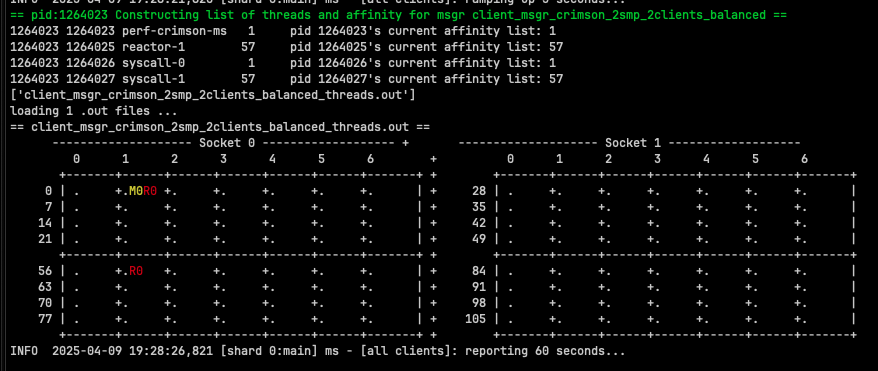
\includegraphics[width=\textwidth]{client_msgr_crimson_2smp_2clients_balanced.png}
  \end{minipage}%
  \caption{CPU Balanced configuration for the Crimson messenger, using two
  cores for server and two cores for the client, respectively.}
  \label{figure:crimson_bal_2}
\end{figure}

\begin{figure}[!ht]
  \centering
  \begin{minipage}{.5\textwidth}
  \centering
    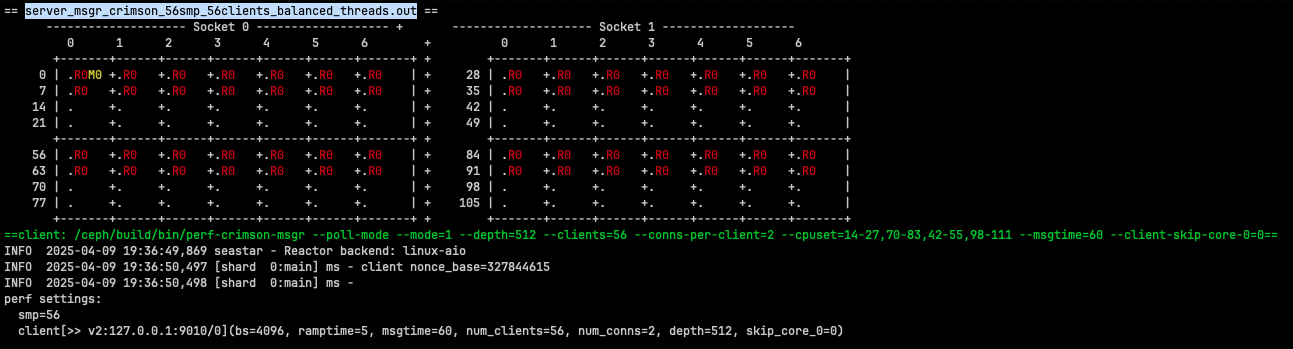
\includegraphics[width=\textwidth]{server_msgr_crimson_56smp_56clients_balanced.png}
  \end{minipage}%
  \begin{minipage}{.5\textwidth}
  \centering
    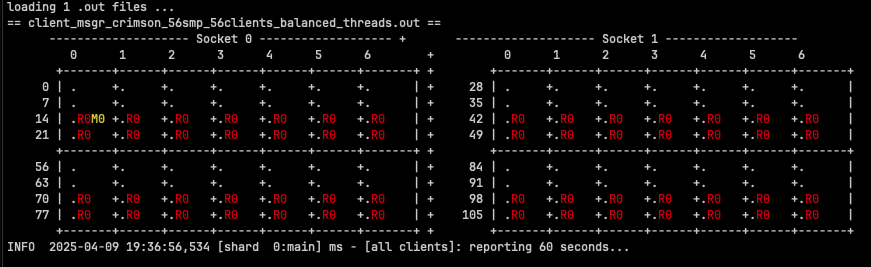
\includegraphics[width=\textwidth]{client_msgr_crimson_56smp_56clients_balanced.png}
  \end{minipage}%
  \caption{CPU Balanced configuration for the Crimson messenger, using 56
  cores for server and 56 cores for the client, respectively.}
  \label{figure:crimson_bal_56}
\end{figure}

In Figure~\ref{figure:crimson_sep_28}, we show theSeparated CPU allocation
where the server only uses physical CPU cores from NUMA socket 0, whereas the
client only uses physical CPU cores from NUMA socket 1. The HT-siblings are not
used in this case. The server and client are using 28 cores each, for a total
of 56 cores.

\begin{figure}[!ht]
  \centering
  \begin{minipage}{.5\textwidth}
  \centering
    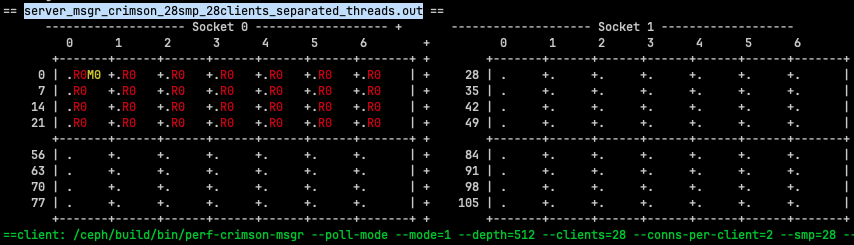
\includegraphics[width=\textwidth]{server_msgr_crimson_28smp_28clients_separated_threads.png}
  \end{minipage}%
  \begin{minipage}{.5\textwidth}
  \centering
    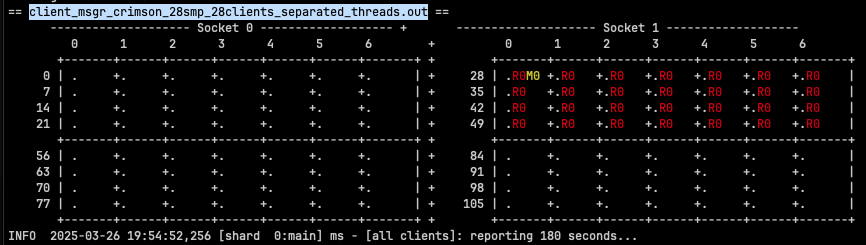
\includegraphics[width=\textwidth]{client_msgr_crimson_28smp_28clients_separated_threads.png}
  \end{minipage}%
  \caption{Separated CPU configuration for the Crimson messenger, using the maximum of 28
  cores for server and 28 cores for the client, respectively.}
  \label{figure:crimson_sep_28}
\end{figure}

In terms of CPU utilisation reported by the client, we can see interesting
differences, for example the following is a snippet of the output of the
Crimson Messenger CPU Separated running 28 clients:
%msgr_crimson_28smp_28clients_separated_client.out

{\small
\begin{verbatim}
1.00516  27043 3.17101e+06  12386.7  8.41057 -- 89,95,95,94,94,95,83,95,95,94,95,96,93,94,95,95,95,94,94,96,96,95,94,95,95,95,95,96,
1.00233  26903 3.17437e+06  12399.9  8.41014 -- 88,95,95,94,94,94,83,94,94,94,95,95,94,94,94,95,94,93,94,96,96,95,94,95,95,95,94,95,
1.00368  26989 3.16918e+06  12379.6  8.39509 -- 89,95,95,93,94,93,83,94,94,94,94,94,94,94,94,94,94,93,94,95,96,95,94,95,95,95,94,95,
1.00298  26925 3.17407e+06  12398.7  8.37066 -- 87,95,95,94,94,93,83,94,94,94,95,94,94,94,95,95,94,94,94,95,96,94,94,95,95,94,94,95,
1.00247  27358 3.17295e+06  12394.3  8.40587 -- 86,95,95,94,94,93,83,93,93,94,94,94,95,95,94,95,94,94,94,95,96,94,94,95,95,94,95,96,
1.00475  26056 3.16877e+06    12378   8.4279 -- 86,94,96,93,94,93,83,93,93,94,94,94,95,94,94,94,93,94,94,95,96,93,94,95,94,94,94,96,
1.00432  27238 3.16835e+06  12376.4  8.37966 -- 86,94,96,93,94,93,83,93,94,94,94,95,95,94,94,95,93,94,94,95,96,93,94,95,94,94,94,96,
1.00265  27260 3.16951e+06  12380.9  8.43864 -- 87,94,97,94,94,93,82,93,94,94,95,95,95,94,94,95,93,94,94,95,96,93,94,94,95,94,95,96,
1.00237  27751 3.17079e+06  12385.9  8.42701 -- 87,95,96,93,93,93,82,93,93,94,95,95,94,94,94,95,93,93,93,94,95,93,94,94,95,95,95,96,
1.00198  27185 3.16717e+06  12371.7  8.41751 -- 87,95,96,93,93,93,82,92,94,94,95,95,94,94,94,96,93,93,94,95,95,93,94,94,95,95,95,96,
-------------- summary --------------
40.1393     -3.17785e+06 12413.5 8.37097
\end{verbatim}
}

In contrast notice the difference with the output of the same Crimson Messenger
running 28 clients but CPU balanced:
% msgr_crimson_28smp_28clients_balanced_client.out
{\small
\begin{verbatim}
1.01299  27657 2.52677e+06   9870.2  10.7857 -- 87,99,95,82,86,100,99,86,90,98,77,93,89,100,95,94,90,83,100,100,97,83,79,91,76,94,92,95,
1.00414  27005 2.52559e+06   9865.6  10.7712 -- 88,99,96,83,86,100,99,87,89,98,76,92,89,100,95,94,90,83,100,99,97,82,79,91,76,93,92,94,
1.00533  27777 2.53035e+06  9884.17  10.7132 -- 89,99,95,85,86,100,100,86,89,98,77,92,89,100,95,94,91,83,100,100,97,82,79,91,76,94,93,95,
1.00242  27939 2.52323e+06  9856.38  10.8349 -- 89,99,95,84,87,100,100,87,89,98,77,92,89,100,94,95,91,84,100,100,97,83,79,91,76,94,93,95,
1.00228  28079 2.52348e+06  9857.33  10.8177 -- 90,99,95,84,87,100,100,87,90,98,77,92,89,100,94,95,90,83,100,100,97,83,79,90,76,95,93,96,
1.0028  28122 2.52358e+06  9857.72  10.8646 -- 90,99,95,84,87,100,100,87,90,98,77,92,89,100,94,96,90,83,100,99,97,83,79,90,75,94,93,96,
1.0025  28067 2.52335e+06  9856.83   10.816 -- 90,99,95,83,86,100,100,87,90,98,77,93,89,100,94,95,91,83,100,99,97,83,79,90,75,94,93,96,
1.00353  27610 2.52749e+06     9873  10.7239 -- 90,98,95,82,86,100,100,87,90,98,77,93,89,100,94,95,90,82,100,99,97,82,79,90,75,94,92,96,
1.00457  27639 2.52251e+06  9853.55  10.8272 -- 91,98,96,83,86,100,100,86,90,98,77,93,88,100,95,95,90,82,100,99,98,82,79,90,76,94,92,95,
1.00291  27360 2.52387e+06  9858.87  10.8139 -- 91,98,96,82,86,100,100,86,90,99,77,92,89,100,94,95,90,83,99,99,98,82,79,91,76,94,92,95,
-------------- summary --------------
60.2448     -2.52685e+06  9870.5 10.8015
\end{verbatim}
}

Further investigation is in progress.
%The results are shown in Figure \ref{fig:crimson_vs_async}.
% \begin{figure}[H]
%   \centering
%   \includegraphics[width=0.8\textwidth]{crimson_vs_async.png}
%   \caption{Crimson vs. Asynchronous Messenger}
%   \label{fig:crimson_vs_async}
% \end{figure}

\section{Resource contention}

As a first hypothesis, we can venture the possibility of a resource contention
when increasing the number of clients and hence CPU cores for the server. To
support this, we compare the performance between a single instance running 28
cores vs. two instances, each running 14 cores.

(For lack of better name, we have instances named 'left' and 'right', the summary execution results are shown below)
{\small
\begin{verbatim}
== leftmsgr_crimson_14smp_14clients_balanced_client.out ==
all(depth=14336):
  connect time: 0.002588s
  messages received: 89683481
  messaging time: 60.207390s
  latency: 9.153140ms
  IOPS: 1489575.942583
  out throughput: 5818.656026MB/s

== leftmsgr_crimson_14smp_14clients_separated_client.out ==
all(depth=14336):
  connect time: 0.001723s
  messages received: 120069445
  messaging time: 60.212315s
  latency: 6.414321ms
  IOPS: 1994101.163976
  out throughput: 7789.457672MB/s  <--

== rightmsgr_crimson_14smp_14clients_balanced_client.out ==
all(depth=14336):
  connect time: 0.002610s
  messages received: 89745195
  messaging time: 60.203232s
  latency: 9.115692ms
  IOPS: 1490704.014876
  out throughput: 5823.062558MB/s

== rightmsgr_crimson_14smp_14clients_separated_client.out ==
all(depth=14336):
  connect time: 0.001850s
  messages received: 120923772
  messaging time: 60.240741s
  latency: 5.980266ms
  IOPS: 2007342.022439
  out throughput: 7841.179775MB/s <--

\end{verbatim}
}

Compare this figures against a single instance running 28 cores:

{\small
\begin{verbatim}
== msgr_crimson_28smp_28clients_balanced_client.out ==
all(depth=28672):
  connect time: 0.004654s
  messages received: 152236774
  messaging time: 60.247898s
  latency: 10.910158ms
  IOPS: 2526839.747163
  out throughput: 9870.467762MB/s

== msgr_crimson_28smp_28clients_separated_client.out ==
all(depth=28672):
  connect time: 0.003748s
  messages received: 191154296
  messaging time: 60.196743s
  latency: 8.430074ms
  IOPS: 3175492.177325
  out throughput: 12404.266318MB/s <  7789.457672MB/s + 7841.179775MB/s  = 15630 MB/s
\end{verbatim}
}

This suggest that the issue is software related and such a large difference (26\%) should be visible in perf.

We need to examine the profiles (flamegraphs) for comparison of the following CPU profiles:

\begin{itemize}
  \item single instance (28 cores)
    \texttt{msgr\_crimson\_28smp\_28clients\_separated\_client.out} versus dual
    instances of 14 cores, on both cases using the Separated NUMA allocation.
    This is expected to show the resource contention that occurs when the
    number of cores increases.
  \item single instance at the sweet spot (i.e., the highest performance) which
    is 16 cores, using the Separated NUMA allocation, versus the corresponding
    using the Balanced allocation. This should reveal the difference in
    performance between the two CPU allocation strategies.
  \end{itemize}

% between Separated vs. Balanced, using the same number of clients and cores. 
